

\begin{Exercice}[5 minutes]\textbf{Maxim}
Quelle est la forme simplifiée de l’expression suivante?

$$ (p \land q) \lor (\lnot p \land q) \lor (p \land r) $$

\begin{itemize}
    \item $q \lor (p \land r)$
    \item $p \lor q \lor r$
    \item $q \lor r$
    \item $q$
\end{itemize}

\begin{solution}
Option A. 
\end{solution}
\vspace*{0.3cm}
Soit le code Java ci-dessous. Par quelle instruction faut-il remplacer la ligne \#LINE REMOVED pour que les deux fonctions renvoient le même résultat?
\begin{lstlisting}[style=javastyle]
class Foo { 
    public static boolean test1(int x){ 
        if (x % 4 == 0) return true; 
        else if (x % 2 == 0) return false; 
        else return true;
    } 
    public static boolean testAlt(int x){ 
        #LINE REMOVED 
    } 
}
\end{lstlisting}

\mcqlist{
    {\texttt{return (x \% 4 == 0) || (x \% 2 != 0);}},
    {\texttt{return (x \% 4 == 0) \&\& (x \% 2 != 0); }},
    {\texttt{return (x \% 4 != 0) || (x \% 2 == 0);}},
    {\texttt{return (x \% 4 != 0) \&\& (x \% 2 == 0);}}
}

\begin{solution}
Option A. 
\end{solution}


\end{Exercice}

% \begin{Exercice}[5 minutes]\textbf{Amina}

% Laquelle des propositions suivantes représente correctement le nombre $5$ en théorie des ensembles?

% \mcqlist{
%     {$\{\varnothing,\{\varnothing\},\{\varnothing,\{\varnothing\}\},\{\varnothing,\{\varnothing\},\{\varnothing,\{\varnothing\}\}\}\}$},
%     {
%         $\{\varnothing,\{\varnothing\},\{\varnothing,\{\varnothing\}\},\{\varnothing,\{\varnothing\},\{\varnothing,\{\varnothing\}\}\},\{\varnothing,\{\varnothing\},\{\varnothing,\{\varnothing\}\},\{\varnothing,\{\varnothing\},\{\varnothing,\{\varnothing\}\}\}\}\}$
%     },
%     {
%         $\{\{\varnothing\},\{\varnothing,\{\varnothing\}\},\{\varnothing,\{\varnothing,\{\varnothing\}\}\}\}$
%     },
%     {
%         $\{\varnothing,\{\varnothing,\{\varnothing,\{\varnothing,\{\varnothing\}\}\}\}\}$
%     }
% }

% \begin{solution}
% Option B.
% \end{solution}

% \end{Exercice}

\begin{Exercice}[5 minutes]
    Lesquelles des propositions suivantes sont vraies? Pour celles qui sont fausses, énoncer leur négation.
    \mcqlist{
        {$\exists x \in \mathbb{N},\ x^2 > 5$},
        {$\forall x \in \mathbb{N},\ x^2 > 5$},
        {$\forall x \in \mathbb{N},\ \exists y \in \mathbb{N},\ y > x^2$},
        {$\exists y \in \mathbb{N},\ \forall x \in \mathbb{N},\ y > x^2$}
    }

\begin{solution}
\begin{enumerate}
    \item $\exists x \in \mathbb{N},\ x^2 > 5$

    Cette proposition est \textbf{vraie}.  
    En effet, par exemple pour $x = 3$, on a $3^2 = 9 > 5$.

    \item $\forall x \in \mathbb{N},\ x^2 > 5$

    Cette proposition est \textbf{fausse}.  
    Par exemple, pour $x = 0$ ou $x = 1$, on a $x^2 \le 5$.

    Sa négation est :
    \[
    \exists x \in \mathbb{N} \text{ tel que } x^2 \le 5.
    \]

    \item $\forall x \in \mathbb{N},\ \exists y \in \mathbb{N},\ y > x^2$

    Cette proposition est \textbf{vraie}.  
    En effet, pour tout $x \in \mathbb{N}$, le nombre $y = x^2 + 1$ appartient à $\mathbb{N}$ et vérifie $y > x^2$.

    \item $\exists y \in \mathbb{N},\ \forall x \in \mathbb{N},\ y > x^2$

    Cette proposition est \textbf{fausse}.  
    Il n’existe pas de nombre naturel strictement supérieur à tous les carrés $x^2$.

    Sa négation est :
    \[
    \forall y \in \mathbb{N},\ \exists x \in \mathbb{N} \text{ tel que } y \le x^2.
    \]
\end{enumerate}
\end{solution}
\end{Exercice}

\begin{Exercice}[5 minutes]\textbf{Amina}

Considérons le diagramme de Venn suivant, dans lequel A, B, C, D et F représentent des sous-ensembles de E, et où a, b, c, d, e, f, g, h, i sont des éléments de E.

\begin{center}
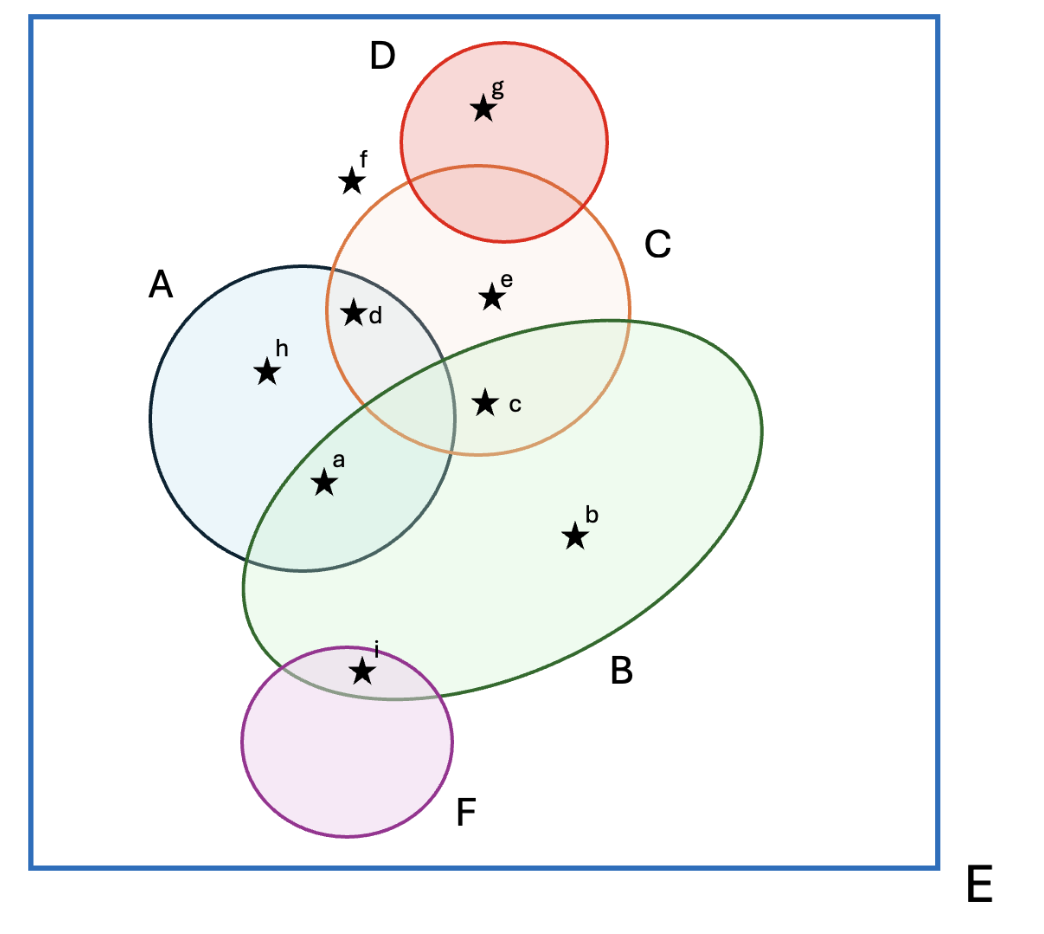
\includegraphics[width=0.6\textwidth]{img/venn.png}
\end{center}


Parmi les assertions suivantes, lesquelles sont correctes? (Plusieurs réponses possibles)

\mcqlist{
    {$d \in (A \cap C) \setminus D$},
    {$c \in (A \cup D) \cap B$},
    {$g \in \overline{A \cup B \cup C}$},
    {$f \in (D \cup C) \cap \overline{A \cup B \cup F}$},
    {$i \in \left(F \cap B \cap \overline{A \cup C \cup D}\right)$},
    {$\{c,e\} \subset (B \cap C) \cup (C \cap D)$},
    {$\{a,i\} \subset B \cap F$},
    {$\{b,c,g\} \subset B \cup D$},
    {
        $\{a,h,i\} \subset (A \cup F) \setminus (C \cap B)$
    }
}
\begin{solution}
Options: A, C, E, H, I. 
\end{solution}

\end{Exercice}

\begin{Exercice}[5 minutes]\textbf{Aurore}
Combien de sous-ensembles contient l'ensemble E = \{1,2,3,4\}?

\mcqlist{
    4, 8, 16, 32
}

\begin{solution}
Option C. Pour un ensemble de $n$ éléments, le nombre de sous-ensembles est donné par $2^n$.
\end{solution}

\end{Exercice}

\begin{Exercice}[5 minutes]\textbf{Aurore}
Dans lesquels des cas suivants la proposition suivante est-elle vraie?
$$
\bigl(((P \land Q) \lor P) \land (\lnot Q \land Q)\bigr)
\lor (\lnot P \land Q)
\lor (P \lor Q)
$$

\mcqlist{
    {$P=V,Q=V$},
    {$P=V,Q=F$},
    {$P=F,Q=V$},
    {$P=F,Q=F$},
    {Aucune de ces réponses n'est correcte}
}

\begin{solution}
A, B, et C.
\end{solution}

\end{Exercice}

\begin{Exercice}[5 minutes]\textbf{Aurore}
Laquelle de ces propositions est vraie par rapport à la classe Java qui débute par la ligne de code suivante:

\lstinline[style=javastyle]{public abstract class Country}
\mcqlist{
    {Elle s'agit d'une interface},
    {Elle peut être instanciée},
    {Elle peut hériter d'une autre classe si le nom est suivi du mot-clé implements},
    {Elle peut contenir des méthodes abstraites},
}

\begin{solution}
Option D. 
\end{solution}

\end{Exercice}
